%********** Chapter 6 **********
\chapter{Camera Transformation Calculation}
\section{Introduction}
In the previous chapter, we explained how to extract feature points from a frame then find matches in the next frame. Now, we explain how we calculate a transformation between the two sets of feature points, this transformation is then applied on the second point cloud to align it with the global point cloud.

Tranformation calculation is a well known mathematical problem, where we calcluate a transformation matrix that when applied to the first set of points will result in the second set of points.

Some of the methods used for transformation calculation are iterative and others are closed form solutions, we have found that applying a closed form solution then using the results as a seed for the iterative solution gives better and faster results than applying only one method.

\section{Horn's method}

We Consider that problem of transforming the second point cloud to the first point cloud identical to the problem of transforming one coordinate system to another, this problem is named the Absolute Orientation Problem, we used the closed form solution proposed by Horn.

The transformation between the two coordinate systems is assumed to be rotation and translation, we denote it as $F_{AB} = [R | t]$

\begin{figure}[htb]
\centering
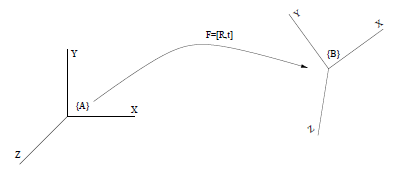
\includegraphics{Transformation_Calc/transformation_AB.png}
\caption{One coordinate system transformed to the other}
\label{fig:transformation_AB}
\end{figure}

\subsection{Quaternions}
Quaternions are a mathematical object of the form
$$ Q = s + ix + jy + kz = s + v $$
where s, x, y, z $\in$ R, and i, j, k are mutually orthogonal imaginary units with the
following composition rule

\begin{table}[htb]
\centering
\begin{tabular}{ l | l  l  l }
  & i  & j  & k \\ \hline
  i& -1& k & -j\\
  j& -k& -1& i\\
  k& j & -i& -1\\
\end{tabular}
\caption{i,j and k composition rule}
\label{tab:ijkcomposition}
\end{table}

We now define several basic operations on quaternions:
\begin{itemize}
\item Addition and Substraction:
     Given two quaternions $q_1 = (s_1, v_1)$ and $q_2 = (s2, v2)$ their addition/subtraction is defined as
$$q = q_1 + q_2 = (s_1 + s_2, v_1 + v_2)$$
\item Multiplication:
Given two quaternions $q_1 = (s_1, v_1)$ and $q_2 = (s_2, v_2)$ their multiplication is defined as
$$q_1 * q_2 = (s_1 + v_1) * (s_2 + v_2) = s_1s_2 + s_1v_2 + s_2v_1 + v_1 * v_2$$

Then compute:
$$v_1 * v_2 = (iv_{1x} + jv_{1y} + kv_{1z}) * (iv_{2x} + jv_{2y} + kv_{2z})$$
$$ = (-v_{1x}v_{2x} - v_{1y}v_{2y} - v_{1z}v_{2z}) +$$
$$ i(v_{1y}v_{2z} - v_{1z}v_{2y}) + $$
$$ j(v_{1z}v_{2x} - v_{1x}v_{2z}) + $$
$$ k(v_{1x}v_{2y} - v_{1y}v_{2x}) $$
$$ = -(v_1 \cdot v_2) + (v_1 \times v_2) $$

Then
$$ q = q_1 * q_2 = [(s_1s_2 � v_1 \cdot v_2);(s_1v_2 + s_2v_1 + v_1 \times v_2)]$$

\end{itemize}

We have just defined quaternions and their basic operations, let's explain how they work as rotation operators

Let's first explain how rotations are expressed using Euler angles then we talk about the problem of gimbal lock and how quaternions avoid it.

Euler angles represent a 3D rotation as a rotation around the 3D axes $x,y $ and $z$, so a rotation is expressed as:

$$ R_{AB} = R_z(\omega_z)R_y(\omega_y)R_x(\omega_x)$$
$$ = 
\begin{bmatrix}
   \cos(\omega_z) & -\sin(\omega_z) & 0 \\
   \sin(\omega_z) & \cos(\omega_z) & 0 \\
   0 & 0 & 1 \\
\end{bmatrix}
\begin{bmatrix}
   \cos(\omega_y) & 0 & \sin(\omega_y) \\
   0 & 1 & 0 \\
   \sin(\omega_y) & 0 & \cos(\omega_y) \\
\end{bmatrix}
\begin{bmatrix}
	1 & 0 & 0 \\
   0 & \cos(\omega_x) & \sin(\omega_x) \\
   0 & \sin(\omega_x) & \cos(\omega_x)  \\
\end{bmatrix}
$$

\normalsize
$$ = 
\begin{bmatrix}
   \cos(\omega_z)\cos(\omega_y) & \cos(\omega_z)\sin(\omega_y)\sin(\omega_x) - \sin(\omega_z)\cos(\omega_x) & \cos(\omega_z)\sin(\omega_y)\cos(\omega_x) + \sin(\omega_z)\sin(\omega_x)  \\
   \sin(\omega_z)\cos(\omega_y) & \sin(\omega_z)\sin(\omega_y)\sin(\omega_x) + \cos(\omega_z)\cos(\omega_x)  &  \sin(\omega_z)\sin(\omega_y)\cos(\omega_x) - \sin(\omega_z)\sin(\omega_x)  \\
   -\sin(\omega_y) &  \cos(\omega_y)\sin(\omega_x)  & \cos(\omega_y)\cos(\omega_x) \\

\end{bmatrix}
$$

\large
\pagebreak
if we have a rotation matrix and want to get the rotation angles around the axes we use the following relations:

$$\omega_y = \mathrm{atan2}(-r_{31}, \sqrt{r_{11}^2 + r_{21}^2}) $$
$$\omega_z = \mathrm{atan2}(r_{21}/\cos{\omega_y}, r_{11}/\cos{\omega_y}) $$
$$\omega_x = \mathrm{atan2}(r_{32}/\cos{\omega_y}, r_{33}/\cos{\omega_y}) $$


the problem of gimbal lock happens when a rotation causes two of the axes are in the same plane, for instance, if $\omega_y = \pi/2$ then we will not be able to extract the angles in the previous relations.


\begin{figure}[htb]
\centering
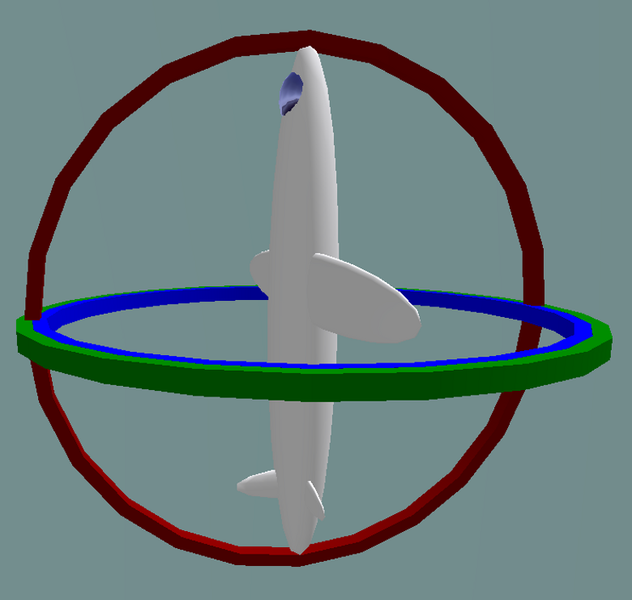
\includegraphics[scale=0.45,keepaspectratio=true]{Transformation_calc/gimbal_lock.png}
\caption{Gimbal lock happens when two rotation axes are in the same plane}
\label{fig:gimbal_lock}
\end{figure}

this happens because Euler angles defines a 3D rotation as 3 rotations around the three axes, which causes a loss of degree of freedoms when two axes are in the same plane, this doesn't happen when we use quaternions because they define rotation around a unit vector not around the three axes $x, y$ and $z$

\pagebreak

The conjugate norm and inverse are given by the following three equations:

$$\bar{q} = [s, -v] $$
$$ N(q) = \| q \| = \sqrt{q * \bar{q}} = \sqrt {s^2 + |v|^2} $$
$$ q^{-1} = \frac{1}{q} = \frac{1}{q} * \frac{\bar{q}}{\bar{q}} = \frac{\bar{q}}{N(q)^2}$$

if $ N(q) = 1 $ then the quaternion is referred to as a unit quaternion and $\bar{q} = q^{-1}$

\subsection{Quaternions as rotational operators}

Given two vectors $a$ and $b$ and a unit quaternion of the form $q = [\cos \frac{\theta}{2}, n \sin \frac{\theta}{2}] $ the general rotation of $a$ into $b$ about an arbitrary unit axis $n$ by $\theta$ radians is given by the equation:

$$ b = q * a * q^{-1} $$
It can be proved that the previous equation is equivalent

\subsection{Closed Form Registration}

Given two sets of corresponding points in two different coordinate systems, we want to compute the transformation between the coordinate systems.
This solution assumes we have at least three correspondences between the two coordinate systems.

For any two corresponding points $p_l$ and $p_r$, the error in the tranformation can be defined as:
$$ e_i = p_r - R(p_l) - t $$

We want to minimize the sum of square errors over all points:
$$\sum_{i=1}^{n} \| e_i \| ^ 2$$

We will refer all measurements to the centroids given by:
$$ \mu_l = \frac{1}{n} \sum_{i=1}^{n} p_{l,i} $$
$$ \mu_r = \frac{1}{n} \sum_{i=1}^{n} p_{r,i} $$

The new coordinates are now:
$$ p'_{l,i} = p_{l,i} - \mu_l $$
$$ p'_{r,i} = p_{r,i} - \mu_r $$

the error term using the new coordinates becomes
$$ e_i = p'_r - R(p'_l) - t' $$
where
$$ t' = t - \mu_r + R\mu_l$$

The sum of square errors becomes
$$\sum_{i=1}^{n} \| e_i \| ^ 2 = \sum_{i=1}^{n} \|  p'_r - R(p'_l) - t' \| ^ 2$$
$$ = \sum_{i=1}^{n} \|  p'_r - R(p'_l) \| ^ 2 - 2t' \cdot \sum_{i=1}^{n}[p'_{r,i} - Rp'_{l,i}] + n\|t'\|^2 $$

Because $\sum_{i=1}^{n} p'_{r,i} = \sum_{i=1}^{n} p'_{l,i} = 0$ we notice that the middle term in the previous equation equals zero, we minimize the last term by making it equal to zero then
$$ t' = 0 $$
$$ \downarrow $$
$$ t = \mu_r - R\mu_l $$

We have now to minimize the first term
$$ \sum_{i=1}^{n} \|  p'_r - R(p'_l) \| ^ 2 = \sum_{i=1}^{n} \| p'_{r,i} \| ^ 2 - 2 \sum_{i=1}^{n} p'_{r,i} \cdot Rp'_{l,i} + \sum_{i=1}^{n} \| Rp'_{l,i} \| ^ 2$$

The first and third terms of the previous equation are constants independent of R because rotations preserve the vector norm. We minimize the error by maximizing the second term.

This can be expressed in the following figure:
\begin{figure}[htb]
\centering
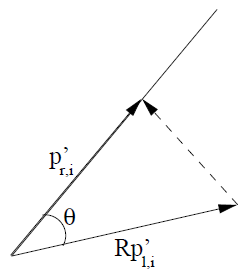
\includegraphics{Transformation_calc/gemoetric_int.png}
\caption{Maixmizing the sum $ \sum{i=1}^{n} p'_{r,i} \cdot Rp'_{l,i} $ is equivalent to maximizing $ \sum{i=1}^{n} | p'_{r,i} | |Rp'_{l,i}| \cos\theta $. This sum is maximized when $\cos\theta = 1$, $\theta=0$. Gemoetrically we compute the rotation which minimizes the angle between the two vectors}
\label{fig:gemoetric_int}
\end{figure}

We express the equation using unit quaternions:
$$ \sum{i=1}^{n} (q * p'_{l,i} * \bar{q}) \cdot p'_{r,i} $$
$$ = \sum{i=1}^{n} (q * p'_{l,i}) \cdot (p'_{r,i} *q) $$

We use the matrix representation:

$$p'_{r,i} * q = \begin{bmatrix}
   0 & -x'_{r,i} & -y'_{r,i}& -z'_{r,i} \\
   x'_{r,i} & 0 & -z'_{r,i} & y'_{r,i} \\
   y'_{r,i}& z'_{r,i} & 0 & -x'_{r,i}  \\
   z'_{r,i} & -y'_{r,i} & x'_{r,i} & 0  \\
\end{bmatrix}q = \Re_{r,i}q $$

and

$$q * p'_{l,i} = \begin{bmatrix}
   0 & -x'_{l,i} & -y'_{l,i}& -z'_{l,i} \\
   x'_{l,i} & 0 & z'_{l,i} & -y'_{l,i} \\
   y'_{l,i}& -z'_{l,i} & 0 & x'_{l,i}  \\
   z'_{l,i} & y'_{l,i} & -x'_{l,i} & 0  \\
\end{bmatrix}q = \bar{\Re_{l,i}}q $$

So we have:

$$ \sum{i=1}^{n} (\bar{\Re_{l,i}}q) \cdot (\Re_{r,i}q) $$
$$ \Downarrow $$
$$ \sum{i=1}^{n} q^T\bar{\Re_{l,i}}^T \Re_{r,i}q $$
$$ \Downarrow $$
$$ q^T (\sum{i=1}^{n} \bar{\Re_{l,i}}^T \Re_{r,i})q $$
$$ \Downarrow $$
$$ q^T (\sum{i=1}^{n} N_i) q $$
$$ \Downarrow $$
$$ q^T N q$$

The matrix $N$ is symmetric as it is a sum of symmetric matrices. The vector $q$ which maximizes $q^TNq$ is the eigenvector corresponding to the most positive eigenvalue of the matrix $N$.

We construct the matrix N by:
$$ M = \sum{i=1}^{n} p'_{l,i}p{'T}_{r,i}$$
$$ = \sum{i=1}^{n} [p_{l,i}p_{r,i}^T] - \mu_l\mu_r^T$$
$$ = \begin{bmatrix}
   S_{xx} & S_{xy} & S_{xz} \\
   S_{yx} & S_{yy} & S_{yz} \\
   S_{zx} & S_{zy} & S_{zz}  \\
\end{bmatrix}$$
where
$$ S_{xx} \sum{i=1}^{n} x'_{l,i}x'_{r,i} $$
$$ S_{xy} \sum{i=1}^{n} x'_{l,i}y'_{r,i} $$
and so on. The matrix contains all the information needed to construct the matrix N
$$ N =  \begin{bmatrix}
   trace(M) & \Delta^T \\
   \Delta & M + M^t - trace(M)I_3 \\
\end{bmatrix}$$ 
where
$$ N =  \begin{bmatrix}
   (M - M^T)_{23} \\
   (M - M^T)_{31} \\
	(M - M^T)_{12} \\
\end{bmatrix}$$

\subsection{Results of Horn's method}

We have successfully implemented the previously explained method, and have reached results that (measure time of horn)
We noticed that this method works well when:
\begin{itemize}
\item The two frames are rich in features, meaning they have a high (specific) number of matches.
\item The features must also be well distributed over the image space, meaning that features are not only focused in one place in the two images.
\end{itemize}

if one or both of these conditions fail to exist, the results will not be correct and what happens is that the transformation calculated will be biased towards the feature points used in the calculations, this means that these features will be aligned well but the rest of the scene may or may not align in the right place.

This problem occurs a lot when the scanned scene contains a large continous space of the same surface like walls or floors, these surfaces don't contribute in the feature tracking thus are not considered in the transformation calculations, this is explained in the following images:


\begin{figure}[htb]
\centering
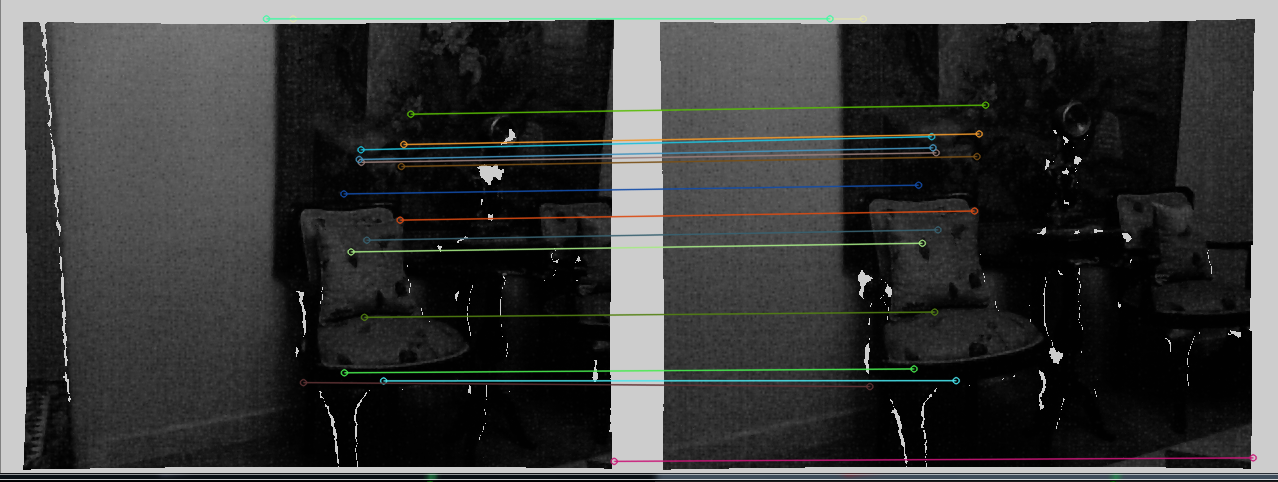
\includegraphics[scale=0.5, width =150mm,keepaspectratio=true]{Transformation_calc/matches_chairs.png}
\caption{We notice that most features are concentrated in the parts that contains chairs while the wall on the right has no features matched}
\label{fig:matches_chairs}
\end{figure}

this causes the transformation to be baised towards the chairs while neglecting the alignment of the walls

\begin{figure}[htb]
\centering
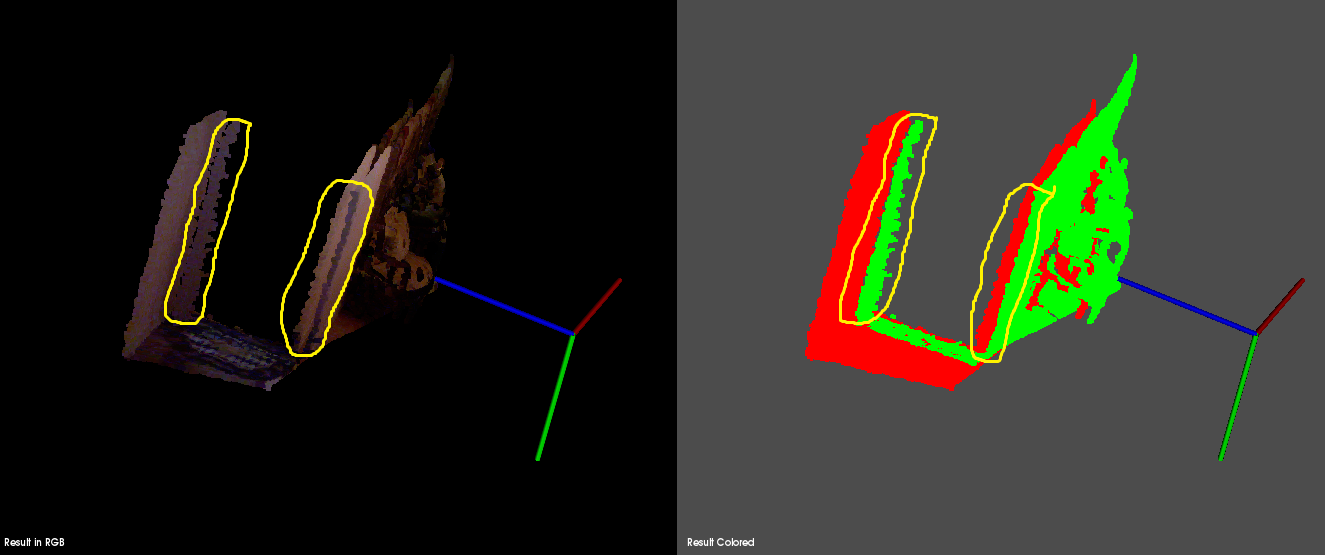
\includegraphics[height=100mm,width=150mm]{Transformation_calc/chairs_horn.png}
\caption{Areas marked with yellow show how alignment fails in featureless areas}
\label{fig:chairs_horn}
\end{figure}

As a result of the previous conclusion we used a different transformation estimation algorithm known as Iterative Closest Point (ICP), the following section explains how the algorithm works and the results we have reached.


\section{Iterative Closes Point}

\subsection{Definition}
The Horn's method explained in the previous section was a closed form solution, here we explain ICP which is an iterative algorithm that works as follows:
\begin{enumerate}
\item Find closest neighbour to every point
\item Compute transformation that minimizes the error over all pairs of points
\item Apply transformation and update point cloud
\item Go back to step 1 till stopping criteria is met
\end{enumerate}

\begin{figure}[htb]
\centering
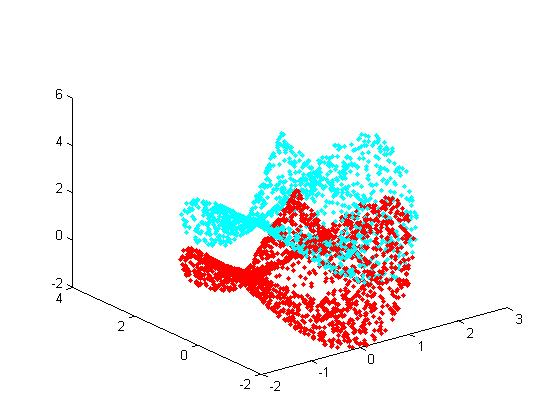
\includegraphics[scale=0.5,keepaspectratio=true]{Transformation_calc/icp.jpg}
\caption{Iterative closest point used to align two point clouds}
\label{fig:icp}
\end{figure}

\subsection{Motivation}
ICP can be used to align two point clouds by iteratively computing the transformation that minimizes the sum of square errors, the problem is that ICP is suffers from:
\begin{itemize}
\item ICP may not converge so we need to set a stopping criteria.
\item ICP may converge to a local minimum, meaning that we may get a transformation that is good but not the best one.
\item ICP is extremely slow as it uses all the points of the point clouds, while Horn's method uses much less number of points, and can do with only three.
\end{itemize}

As stated in the previous chapter, the problem with the closed form solution is that it considers only feature points in transformation calculation, so we decided to use ICP as a second step after obtaining the closed form solution, and we use the obtained transformation as an initial guess to the ICP, this way the ICP step takes less time and converges better, we also consider downsampling the input point clouds to reduce the input size of the ICP making it more faster.

\subsection{Downsampling}

Downsampling is used to reduce the number of points in a point cloud without losing much details.

We use voxel grids to downsample the input point clouds, voxel grids work by dividing the input cloud into small 3D boxes and then replacing every box with the average of all points inside it, the dimensions of the 3D boxes used determine the downsampling ratio, so if we use large boxes we get fewer points and vice versa.

We use a voxel grid of size $(2.5)^3$ $cm^3$, this allows us to reduce the number of points processed in ICP while not losing much of the details of the scene.

\begin{figure}[H]
\centering
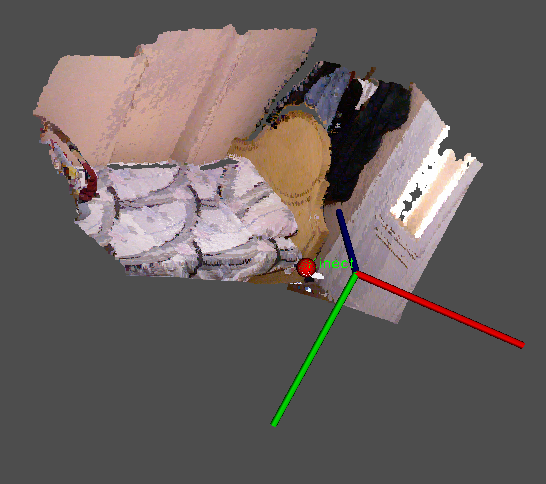
\includegraphics{Transformation_Calc/notDownsampled.png}
\caption{A QVGA scene of a bed without downsampling}
\label{fig:downsample}
\end{figure}

\begin{figure}[H]
\centering
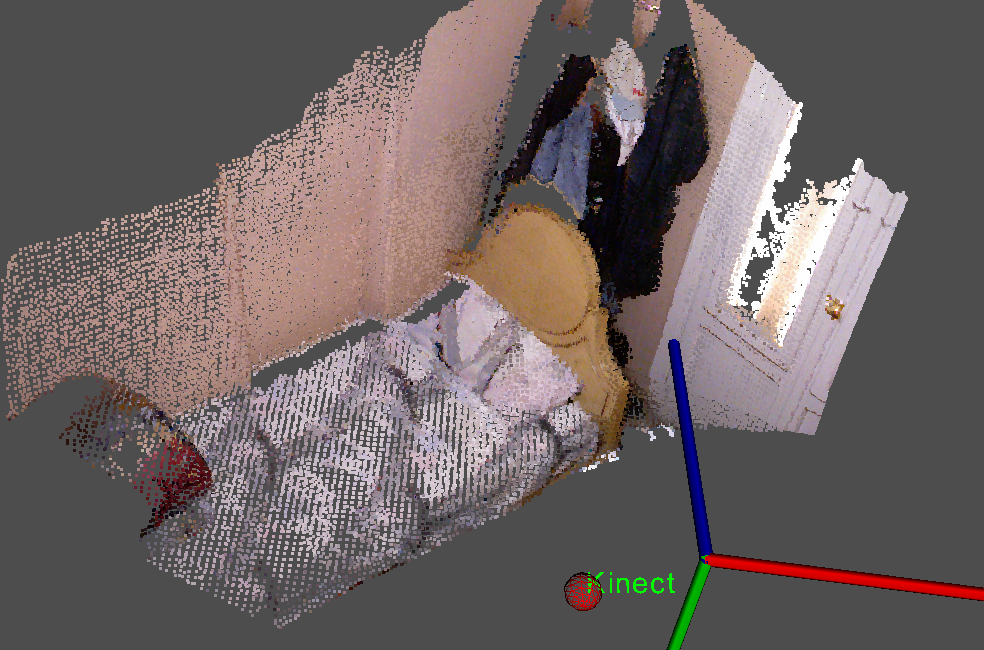
\includegraphics[scale=0.5,keepaspectratio=true]{Transformation_Calc/downsampled.png}
\caption{A QVGA scene of a bed after downsampling}
\label{fig:downsample}
\end{figure}

\pagebreak
\subsection{Results of applying ICP}

After using Horn's method transformation as an initial guess for the ICP procedure on the two downsampled point clouds we have obtained great results because the ICP takes all points in consideration.


\begin{figure}[H]
\centering
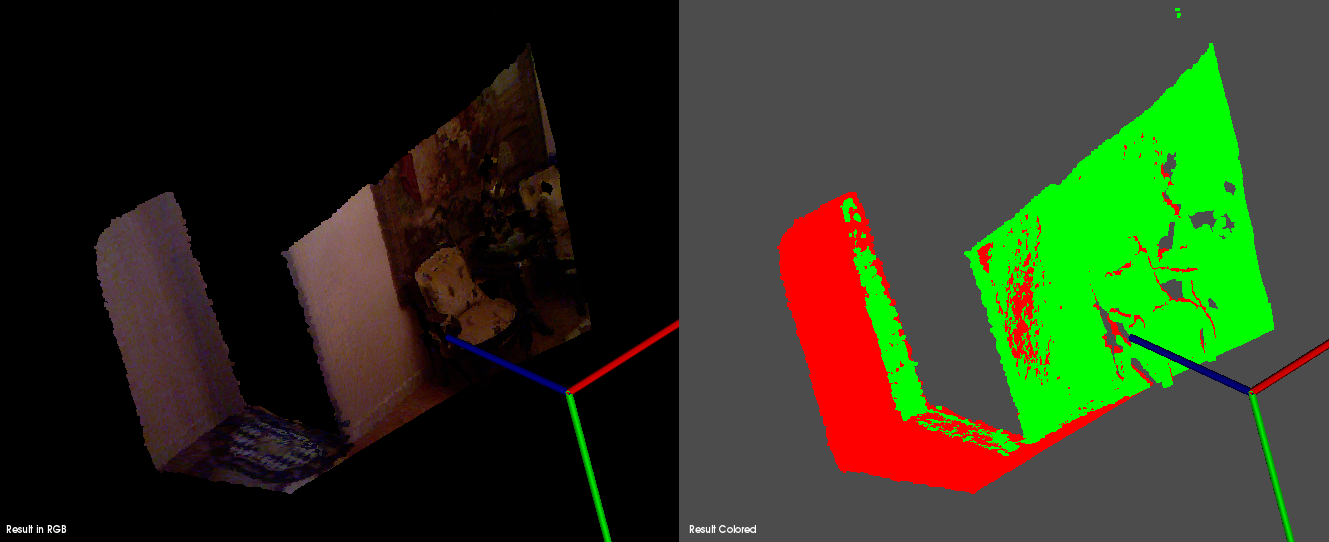
\includegraphics[height=100mm,width=150mm]{Transformation_Calc/chairs_final.png}
\caption{Applying ICP after using Horn's method result as an initial guess, the results are clearly better than the one obtained only with Horn's method in Figure ~\ref{fig:chairs_horn} }
\label{fig:chairs_final}
\end{figure}

The previous figure clearly shows how the results have imporved as we see the two point clouds are well aligned with no gaps, and we notice that the problem that was happening for the wall has disappeared.


\section{Results and performance}

Our system needs is real-time systsm as it needs to provide the constructed 3D model while the user is scanning the environment, this constranis that the alignment takes no more than 2 seconds so that the user will feel no lag in the scanning process.

The performance of the methods we have proposed before satisfy this time constraing as the whole alignment process starting from feature detection to that concatenation of aligned two point clouds takes a maximun of one second for two frames of QVGA resolution. The average time for the alignment is $0.1428$ seconds. [need to do samples and stuff]

We provide here the results obtained from aligning 21 QVGA frames:

\begin{figure}[H]
\centering
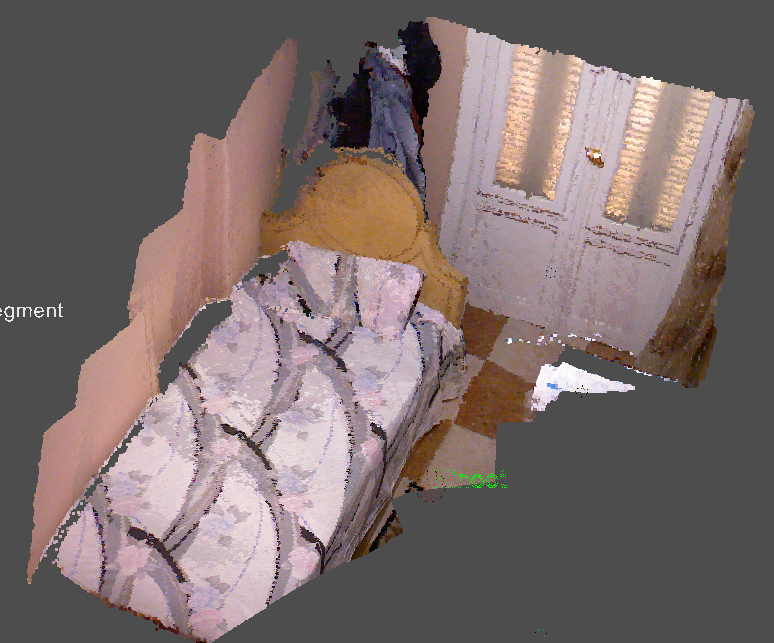
\includegraphics[scale=0.6,keepaspectratio=true]{Transformation_Calc/QVGA1.png}

\label{fig:resultsQVGA_1}
\end{figure}

\begin{figure}[H]
\centering
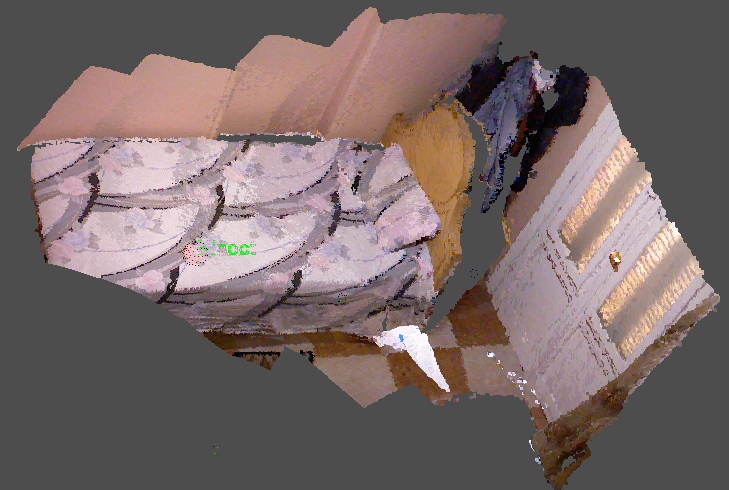
\includegraphics[width=150mm]{Transformation_Calc/QVGA2.png}
\caption{Constructed scene from two different viewpoints}
\label{fig:resultsQVGA_2}
\end{figure}

More accurate results can be obtained by using VGA resolution instead of QVGA, this enhances every step in the alignment process, as the feature detection and tracking is richer, also the ICP operates on more points that describe the scene in more details.

\pagebreak
The difference can be clearly noticed in the two following images that show the alignment result of 14 VGA frames in 7 seconds.

\begin{figure}[H]
\centering
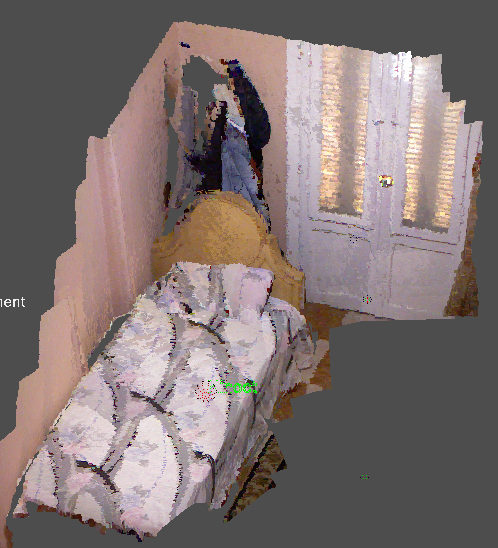
\includegraphics{Transformation_Calc/VGA1.png}

\label{fig:resultsVGA_1}
\end{figure}

\begin{figure}[H]
\centering
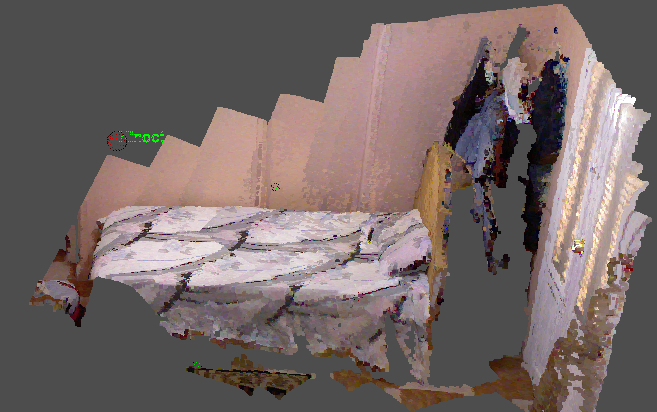
\includegraphics{Transformation_Calc/VGA2.png}
\caption{Constructed scene from two different viewpoints}
\label{fig:resultsVGA_2}
\end{figure}









